\documentclass[12pt,a5paper]{article}
\usepackage[margin=19mm,paperwidth=312mm,paperheight=210mm]{geometry}
\usepackage[italian]{babel}
\usepackage[utf8]{inputenc}
\usepackage[T1]{fontenc}
\usepackage[sc]{mathpazo} % Palatino
\usepackage{lmodern} % Latin modern
\renewcommand*\rmdefault{ppl} %Palatino
\linespread{1.05}
\usepackage{graphicx}
\usepackage{tikz}
\usetikzlibrary{calc}
\usetikzlibrary{positioning}
\usepackage{fix-cm}
\usepackage{lipsum}
\usepackage{lettrine}

\def\lunghezzapagina{148.7mm}
\def\larghezzalaterale{15mm}

\definecolor{mio-verde}{rgb}{0.03, 0.47, 0.19}
\definecolor{mio-azzurro}{HTML}{6ea8b6}
\parindent=0pt

\begin{document}
\pagestyle{empty}

\newsavebox\Blurbbox
\sbox\Blurbbox{\begin{minipage}{110mm}
\lettrine[lines=4]{È}{} davvero un onore, per me, presentarvi questo opuscoletto in memoria e celebrazione dei
50 anni della nostra bella parrocchia di s. Francesco. Nella riunione del Consiglio Parrocchiale 
abbiamo raccolto alcune idee per celebrare e ricordare questo avvenimento, che cade giusto nella 
festa del nostro Patrono. E perché non riportare anche per iscritto i momenti salienti della crescita 
(strutturale, pastorale e spirituale) di una comunità di cristiani? E così è nato questo libricino, con 
l’unico intento di raccontare il cammino della comunità di san Francesco, attraverso i suoi 
protagonisti ancora viventi: pastori e fedeli.
Il libretto che avete per le mani è lungi dall’essere una descrizione esaustiva ed ordinata di 
quanto è avvenuto nel territorio e nel cuore della gente: dovrete aspettare qualche altro buon 
parroco più dotato, paziente e libero del sottoscritto.
Qui ci limitiamo a presentarvi: la “Lettera fondazionale” della parrocchia, con la convenzione tra la 
Diocesi di Trieste e la Provincia religiosa dei Frati Minori Conventuali; l’augurio del Vescovo 
Santin; la Planimetria, con l’elenco aggiornato delle vie e dei numeri civici appartenenti alla 
parrocchia (sostanzialmente tolti dalla parrocchia di san Giovanni Decollato); il racconto dei parroci  
ancora viventi, delle suore Dimesse e quello di due gruppi di parrocchiani, dividendo il periodo in 
due parti (1967-1990; 1990-2015).
A lode e gloria di Dio!
\begin{flushright}
	\textit{fra Tiberio Zilio}
\end{flushright}
\end{minipage}}

\begin{tikzpicture}[remember picture, overlay]
\node[minimum width=\lunghezzapagina,inner sep=0pt,anchor=east, outer sep=0pt, fill opacity=1.0, align=center] at (current page.east) {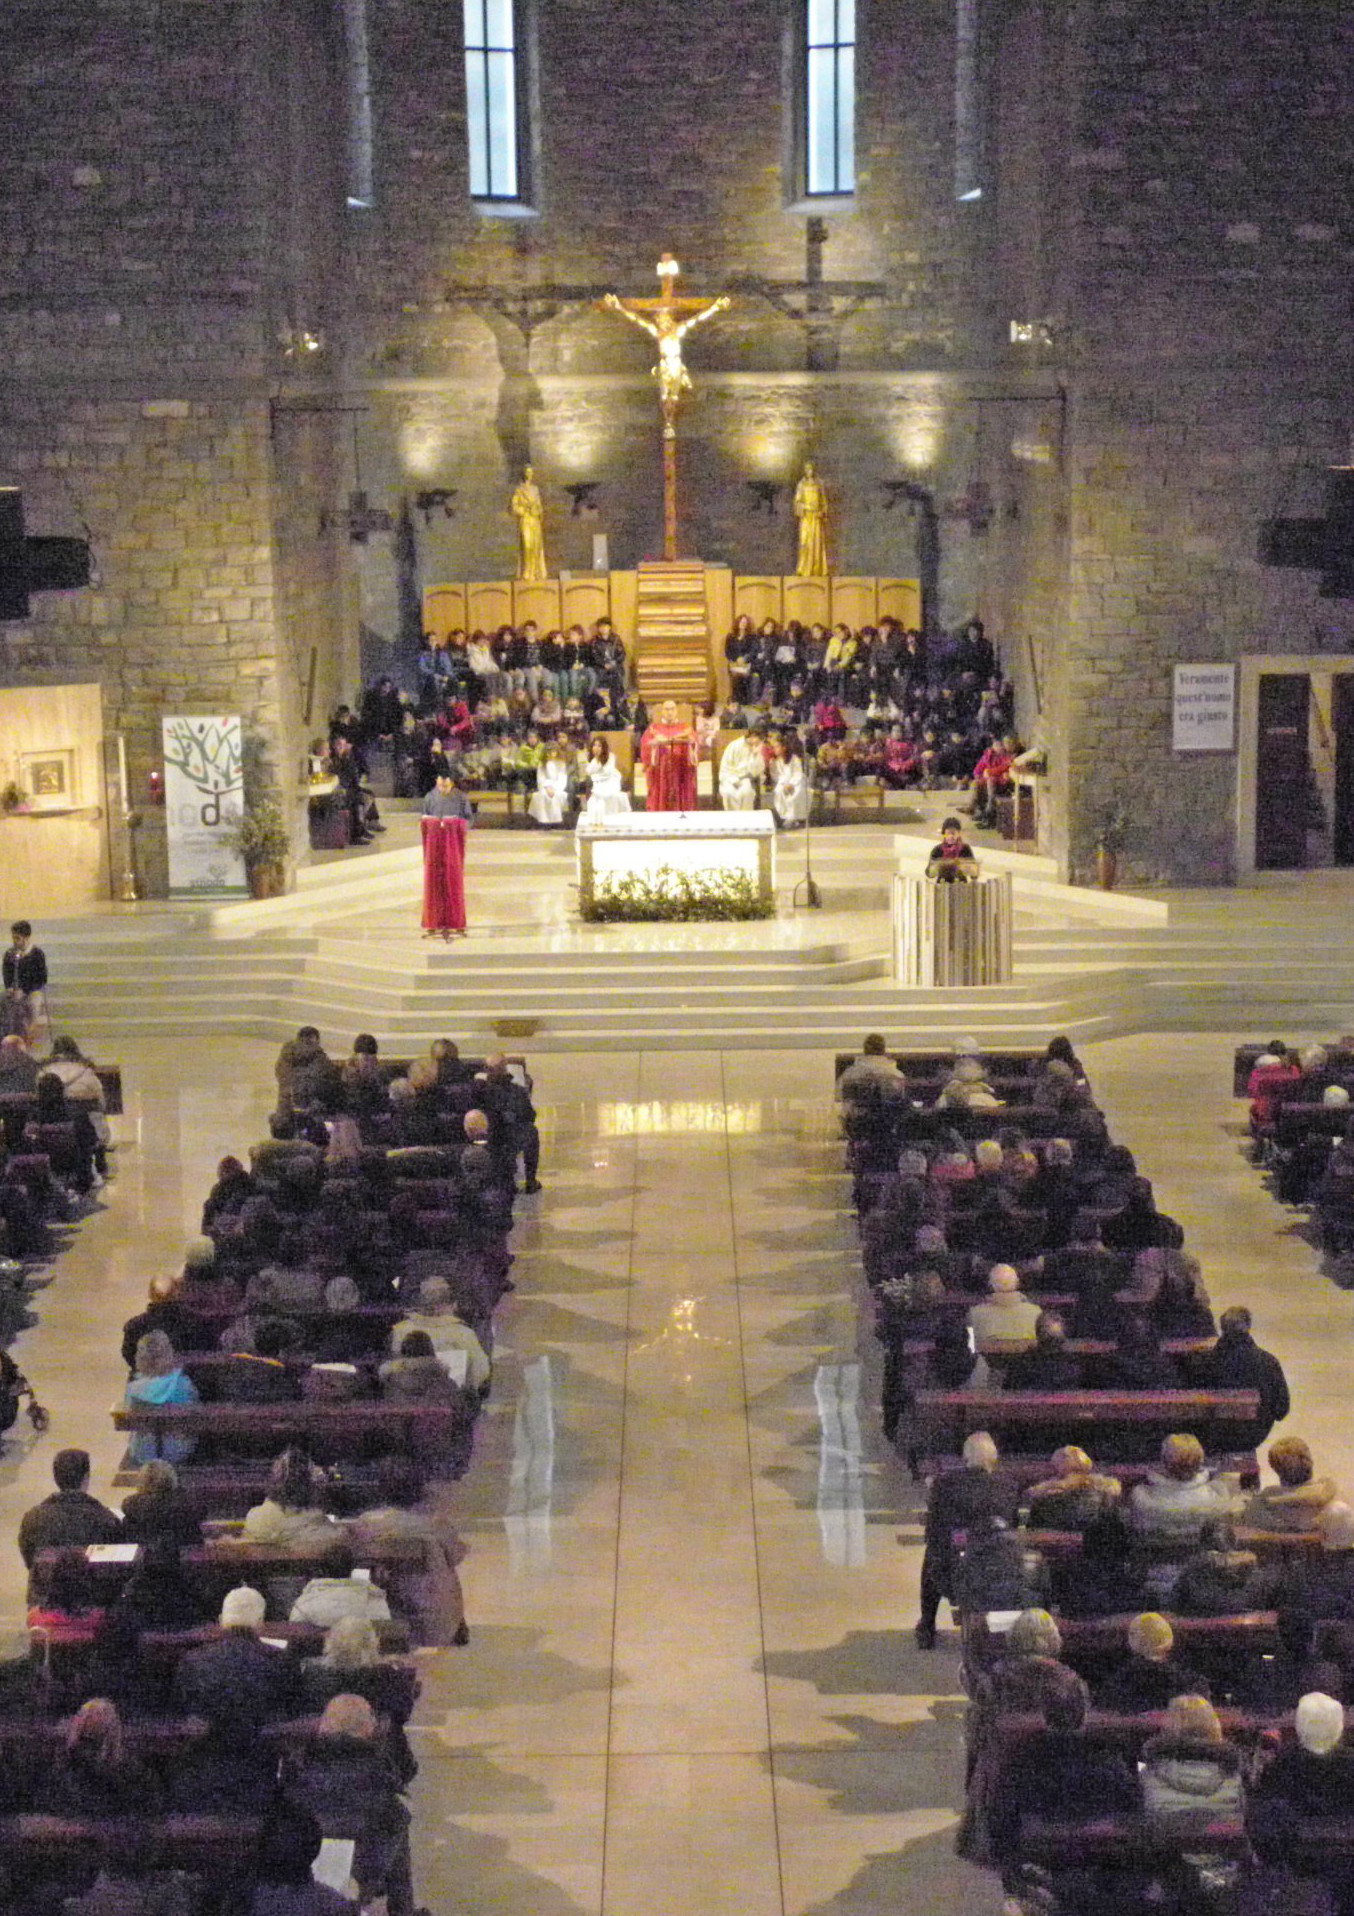
\includegraphics[width=\lunghezzapagina,height=\paperheight]{chiesa}};
\node[text width=\lunghezzapagina,anchor=north east, minimum width=\lunghezzapagina, minimum height=4.5cm, inner sep=0pt, outer sep=0pt, fill=cyan!50, fill opacity=0.7, text opacity=1, align=center] at (current page.north east) {%
\Large{\sffamily PARROCCHIA di SAN FRANCESCO in TRIESTE\par }\bigskip{\fontsize{25}{25}\selectfont\bfseries 2015: 50 ANNI di VITA\par }\bigskip LA COMUNITÀ RACCONTA\par 
};
\node [minimum width=\lunghezzapagina, anchor=south east,align=center,fill opacity=0.3] at (current page.south east) {
\includegraphics[width=8cm]{tau.png}};
\node[text width = \larghezzalaterale,anchor=south, minimum width=\larghezzalaterale, minimum height=\paperheight, inner sep=0pt, outer sep=0pt, fill=mio-azzurro, fill opacity=1, text opacity=1, align=center] at (current page.south) {%
\rotatebox{270}{\bfseries 2015: 50 ANNI di VITA}
};
\node[anchor=west, minimum width=\lunghezzapagina, minimum height=\paperheight, inner sep=0pt, outer sep=0pt, fill=mio-azzurro, fill opacity=1, text opacity=1, align=center] at (current page.west) {%
};
\node[anchor=north west, minimum width=148.6mm,yshift=-19mm, inner sep=0pt, outer sep=0pt,text opacity=1, align=center] at (current page.north west) {%
\usebox\Blurbbox 
};
\end{tikzpicture}

\end{document}
